\documentclass[aspectratio=169]{beamer}



% OPCIONES DE BEAMER

\definecolor{Maroon}{cmyk}{0, 0.87, 0.88, 0.1}
\definecolor{teal}{rgb}{0.0, 0.45, 0.45}

\usetheme[block=fill,numbering=fraction,, subsectionpage=progressbar, titleformat section=smallcaps]{metropolis}
\setbeamertemplate{blocks}[rounded][shadow=false]
\setbeamertemplate{frametitle continuation}[roman]
\setbeamertemplate{section in toc}[balls numbered]
\setbeamertemplate{subsection in toc}[subsections unnumbered]
%\setsansfont[BviejoFont={Fira Sans SemiBold}]{Fira Sans Book}  % Increase font weigth
\widowpenalties 1 10000
\raggedbottom

% COLORES
\setbeamercolor{palette primary}{bg=teal}
\setbeamercolor{progress bar}{use=Maroon, fg=Maroon}

% PAQUETES
\usepackage{bm}
\usepackage{xcolor}
\colorlet{shadecolor}{blue!15}
\usepackage{framed}
\usepackage{amsthm}
\usepackage[utf8]{inputenc}
\usepackage[spanish, es-noshorthands]{babel}
\usepackage{subfig}
\usepackage{graphicx}
\usepackage{minted}
\usepackage{ upgreek }



% Macros
\newcommand{\bx}{\bm{x}}
\newcommand{\bX}{\bm{X}}
\newcommand{\bw}{\bm{w}}
\newcommand{\bW}{\bm{W}}
\newcommand{\bz}{\bm{z}}
\newcommand{\bZ}{\bm{Z}}
\newcommand{\bv}{\bm{v}}
\newcommand{\bV}{\bm{V}}
\newcommand{\bH}{\bm{H}}
\newcommand{\bh}{\bm{h}}
\newcommand{\bSigma}{\bm{\Sigma}}
\newcommand{\bpi}{\bm{\pi}}
\newcommand{\bLambda}{\bm{\Lambda}}
\newcommand{\bmu}{\bm{\mu}}
\newcommand{\btheta}{\bm{\theta}}
\newcommand{\bnu}{\bm{\nu}}
\DeclareMathOperator*{\argmax}{arg\,max}
\DeclareMathOperator*{\argmin}{arg\,min}
\newcommand\E[2]{\mathbb{E}_{#1}\left[#2\right]}
\newcommand\KL[2]{D_{KL}\Big(#1 \bigm|\bigm| #2\Big)}
\newcommand{\bigCI}{\mathrel{\text{\scalebox{1.07}{$\perp\mkern-10mu\perp$}}}}
\newcommand{\bigCD}{\centernot{\bigCI}}
\newcommand{\X}{\mathcal{X}}
\newcommand{\R}{\mathbb{R}}
\usepackage{pgfplots}
%bib

%\bibliography{bibliography.bib}\
%\nocite{*}

\newcommand{\norm}[1]{\left\lVert#1\right\rVert}
\newcommand{\abs}[1]{\left\lvert#1\right\rvert}
\newcommand{\ps}{x^+}
\newcommand{\ns}{x^-}


% TikZ
\usepackage{tikz}

\usepackage{arydshln}
\usepackage{natbib}


\captionsetup[subfloat]{labelformat=empty}

\newtheorem{defi}{Definición}
\newtheorem{prop}{Proposición}
\newtheorem{nth}{Teorema}
\newtheorem{cor}{Corolario}
\newtheorem{ex}{Ejemplo}

\definecolor{studentbrown}{RGB}{124,71,50}
\AtBeginEnvironment{ex}{
    \setbeamercolor{block title}{use=example text,fg=white,bg=example text.fg!75!black}
    \setbeamercolor{block body}{parent=normal text,use=block title example,bg=block title example.bg!10!bg}
}

\usetikzlibrary{arrows.meta,
chains,
positioning}

\newcommand\Fontvi{\fontsize{8}{7.2}\selectfont}

\title{Adversarial Training with Contrastive Learning in NLP}
\subtitle{Procesamiento de Lenguaje Natural}
\date{\today}
\author{Francisco Javier Sáez Maldonado}
\institute{Máster en Ciencia de Datos \\\\\\ \emph{Escuela Politécnica Superior} \\ \emph{Universidad Autónoma de Madrid}}

\usepackage[absolute,overlay]{textpos}


\begin{document}
  \maketitle


  \begin{frame}{Índice}
    \tableofcontents
  \end{frame}

  

  \begin{frame}{Introducción}

    \begin{itemize}
      \item \textbf{Tarea}: Modelado del lenguage (LM) y Traducción automática (NMT)
      \pause 
      \item \textbf{Objetivo}: Conseguir modelos que sean más robustos semánticamente:
      \[
      \text{Inputs parecidos} \implies \text{ Outputs parecidos}  
      \]
    \end{itemize}
  \end{frame}
  

  \section{Herramientas}

  \subsection{Adversarial Training}
  \begin{frame}{Adversarial Training}

    \begin{defi}[Adversarial Learning]
      Técnica usada en el aprendizaje automático para, usando información sobre un modelo, crear ataques maliciosos para causar fallos en el modelo
    \end{defi}
    \pause

    \begin{defi}[Adversarial example]
      Ejemplo diseñado para engañar al modelo, creado introduciendo una \emph{perturbación} en un ejemplo original.
    \end{defi}

    \begin{center}
    ¿ Cómo ayuda el aprendizaje adversario a nuestros modelos ?
    \end{center}

  \end{frame}

  \begin{frame}{Técnicas de creación ejemplos adversarios en NLP}

    \begin{itemize}
      \item Visuales: \citep{DBLP:journals/corr/abs-2005-05909}.
      \begin{table}[H]
        \begin{tabular}{l|l|l}
        Original Input      & This film has a special place in my heart & \textcolor{green}{Positive} \\ \hline
        Adversarial example & This film has a special pl\textcolor{red}{ca}e in my he\textcolor{red}{ra}t & \textcolor{red}{Negative}
        \end{tabular}
        \caption{Ejemplo extraído de \citep{DBLP:journals/corr/abs-1801-04354}}
        \end{table}
      \item Semánticas:\citep{DBLP:journals/corr/abs-1907-11932}
      \begin{figure}[H]
        \centering
        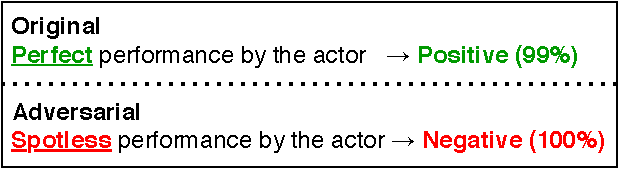
\includegraphics[scale=0.5]{00-ae-example}
        \caption{Ejemplo extraído de \citep{DBLP:journals/corr/abs-1907-11932}}
      \end{figure}

    \end{itemize}
  \end{frame}

  \begin{frame}{Ejemplos adversarios}
    Dada una secuencia \(s = \{x_1,\dots,x_T\}\) de tokens
    \begin{enumerate}
      \item Creamos una representación embebida en un espacio continuo 
      \[
        \mathbf{E}x_i = e_i.  
      \]
      \item Añadimos una pequeña perturbación en el embedding
      \[
      e_i' = e_i - \epsilon \frac{g}{\norm{g}_2},   
      \]
      siendo \(g = \nabla_{e_i}J(s,\theta)\) y \(J\) la función de coste.
    \end{enumerate}

    Función de coste actual:
    \[
    \mathcal J(\theta) = \sum_s \mathcal L(s,\theta) + \alpha \sum_{s'} \mathcal L_{adv} (s',\theta), \quad \alpha \in [0,1].  
    \]
  \end{frame}

  \subsection{Contrastive Learning}

  \begin{frame}{Contrastive Learning}
    
      {\color{Maroon}\textbf{Idea}:} Acercar las representaciones de ejemplos positivos (de la misma clase) y alejar las de los ejemplos negativos (resto de ejemplos).
    

    \begin{ex}
      Original: Elefante. Positivo: Hipopótamo. Negativo: Pistola.
    \end{ex}

    \begin{defi}[Pérdida contrastiva]
      Sean \(a_i\) las entradas originales, \(p_{a_i}\) ejemplos positivos y \(n_{a}\) ejemplos negativos. Se define la pérdida contrastiva como:
      \[
      \mathcal L_{cont} = - \sum_{a_i \in A} \log \frac{\exp(a_i \cdot p_{a_i}/\tau)}{\sum_{n_a \in A - \{ a_i \} } \exp(a_i \cdot n_a / \tau)}  
      \]
    \end{defi}
  \end{frame}


  \section{Framework}

  \begin{frame}{Elementos}
    Consideramos :
    
    \begin{itemize}
    \item  \(\mathbf S = \{s_1,\dots,s_B\}\) un conjunto de frases, donde cada frase \(s_k = \{x_{k1},\dots,x_{kN}\}\) tiene \(N\) tokens.
    \pause
    \item \(\mathbf E s_k = \{\mathbf E x_{k1},\dots, \mathbf E x_{kN}\} = \{e_{k1},\dots e_{kN}\}\) el embedding al espacio continuo de cada frase.
    \pause
    \item El vocabulario \(\mathcal V\) y un subconjunto \textbf{restringido} del mismo del que excluimos palabras incompletas (caracteres individuales o símbolos) \(\mathcal V_R\)
    \pause
    \item La función que nos da la restricción a \(\mathcal V_R\):
    \[
      \mathcal M (\mathbf E x_{ki}) = \begin{cases}1 & \text{ if } x_{ki}\in \mathcal V_R \\ 0 & \text{otherwise}\end{cases}
    \]
    (evita tomar candidatos a modificación adversaria sin sentido).

    \pause
    \item Llamaremos \(h_{kj}\) a la representación obtenida de la frase \(s_k\).

    \end{itemize}
  \end{frame}

  \begin{frame}{Adversarial Training with Contrastive Learning (ATCL)}

    \setbeamercolor{background canvas}{bg=white}
    \begin{figure}
    \centering
    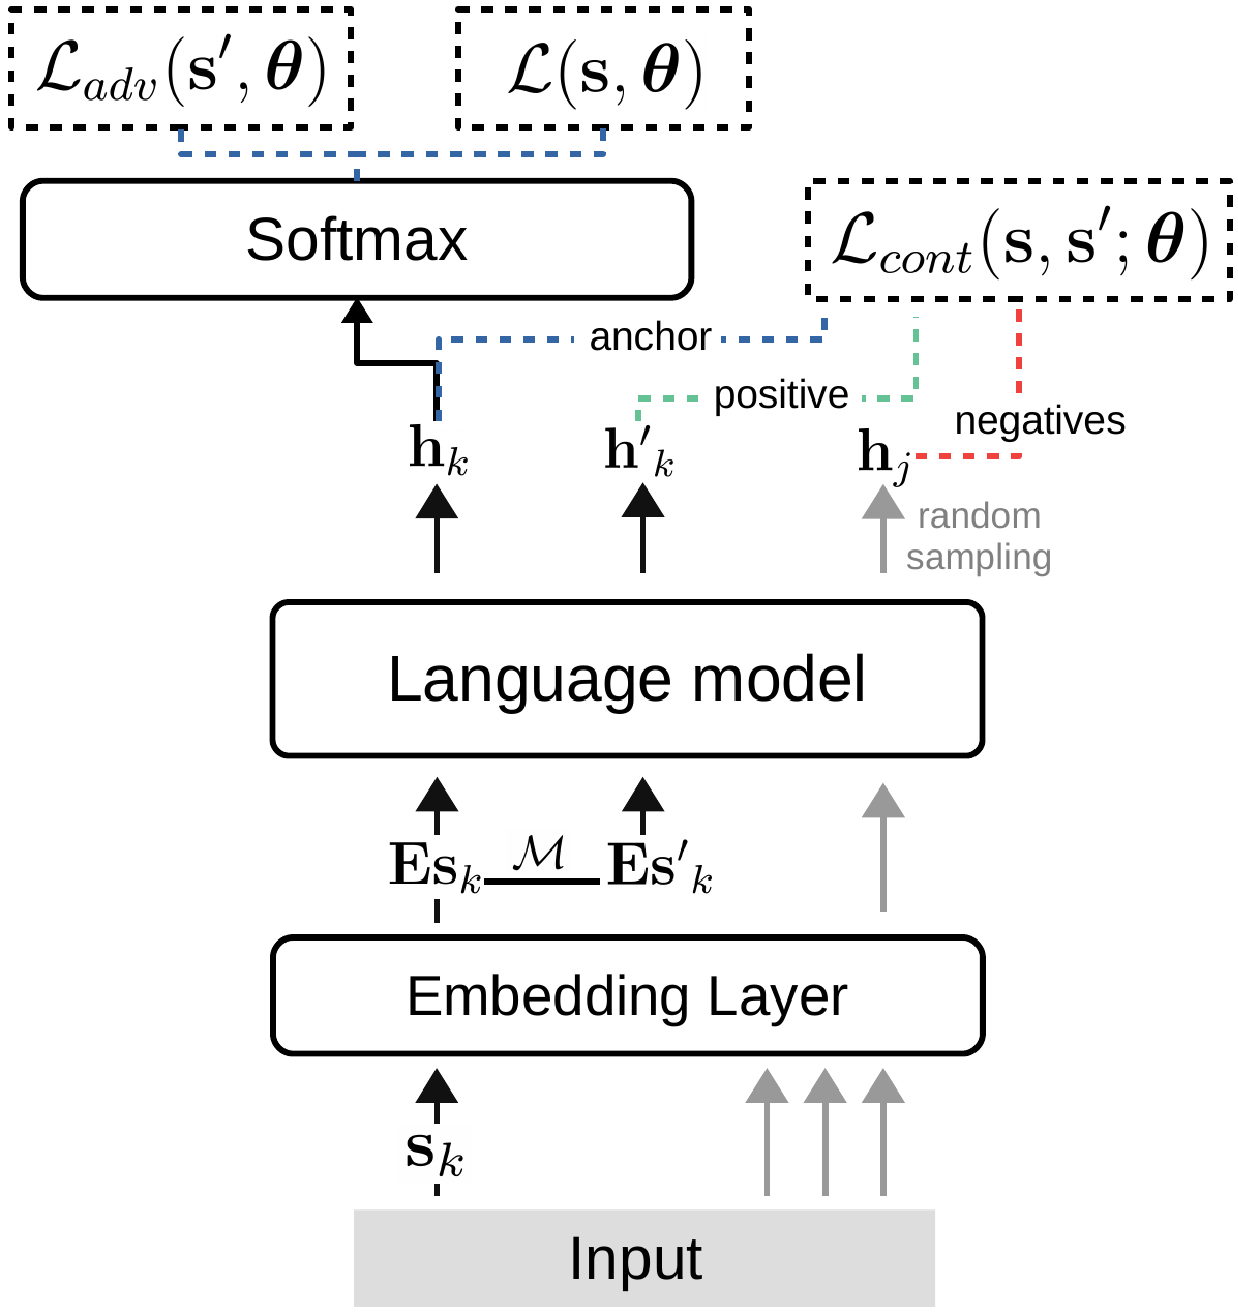
\includegraphics[scale=0.3]{embed}
    \caption{ACTL Framework. Image obtained from the original paper \citep{DBLP:journals/corr/abs-2109-09075}.}
    \end{figure}
  \end{frame}

  \begin{frame}{Consideraciones sobre ATCL}

    
    \begin{itemize}
      \item Con el ejemplo adversario alejamos la representación de la frase original, y forzamos la cercanía mediante contrastive learning.
      
      \item Para la función de pérdida contrastiva, \(\mathcal L_{\text{cont}}\), los ejemplos negativos se samplean del conjunto \(\mathbf{H(S)} - \{h_{kj}\}\), para evitar tomar a la misma \(h_{kj}\) como ejemplo negativo.
    \end{itemize}

    \begin{defi}[Función de pérdida de ATCL]
      La función de pérdida que se utiliza para entrenar el framework ATCL es:
      \[
      \mathcal J(\mathbf \theta)_{\text{ATCL}} = \sum_{\mathbf{s},\mathbf{s'}} \left( \mathcal L + \alpha \mathcal L_{\text{adv}} + \beta \mathcal L_{\text{cont}}\right)  
      \]
    \end{defi}

    \end{frame}

  
  \begin{frame}
  \end{frame}

  \section{Experimentos y resultados}
   PERPLEXITY
   TABLE resultados
   TABLE NEIGHBOURS


  \begin{frame}{Modelo de Lenguaje}
    Datasets:
    \begin{itemize}
      \item Pen Tree-Bank (1M ejemplos)
      \item WikiText-103 (+100M ejemplos)
    \end{itemize}
    
  \end{frame}

  \begin{frame}{Traducción automática}

  \end{frame}

  
  \begin{frame}{Conclusiones}

    \begin{itemize}
      \item omega Yea
    \end{itemize}
  \end{frame}
  
  \appendix

  \begin{frame}[noframenumbering,standout]
    Gracias por su atención
  \end{frame}


  \begin{frame}[noframenumbering]

  \vspace{0.5cm}
  \bibliographystyle{dinat}
  \bibliography{bibliography.bib}

  \end{frame}

\end{document}
